\section{Voice Interface}

After enabling the robot to navigate using ARTags we wanted a simple way to control it and we implemented a Voice Interface. The first step was to find a suitable Automatic Speech Recognizer (ASR); we settled for the Google Speech Recognizer as it currently is one of the best performing over free-form speech and developed and Android application to make use of its API. The goal of this application is to take as input a sound, the spoken commands, and returns a set of possible interpretations to the computer controlling the robot. Figure \ref{fig:tablet_speak} shows the main interface of the application. 

\begin{figure}[h!]
  \centering
    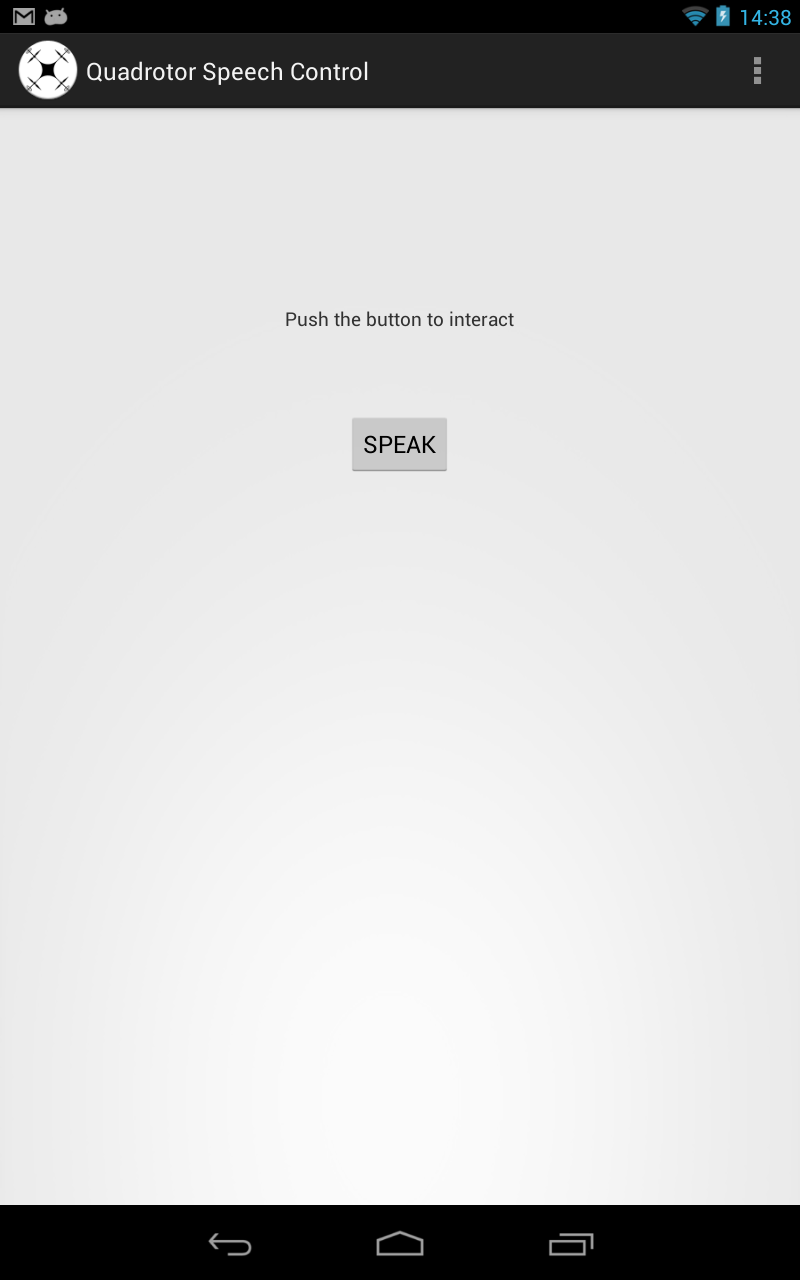
\includegraphics[scale=0.25]{figs/tablet1.png}
  \caption{Main screen from the Android app}
  \label{fig:tablet_speak}
\end{figure}


When using speech to control a robot a wide set of problem arise; first of all people expect from robots to do much more then what they are currently able to, moreover they use many different ways to express the same command and, last, speech recognition technologies often introduce errors in the transcription of the audio input.
%Mettere qui info sul tablet, risultati multipli ecc?


In order to cope with all these problems we first identified a set of behaviors the robot could execute. The resulting list, given that in our simulation we only had the quadrotor move backward and forward, is the following:
\begin{itemize}
\item FORWARD the robot moves to the next tag
\item BACK the robot moves to the previous tag
\item LAST the robot goes to the last tag of the path
\item FIRST the robot goes to the first tag of the path
\item STOP if the robot is going to the first or last tag it will stop and hover on the current tag
\end{itemize}
As first naive approach was to check if the output of the Speech Recognizer contained the keyword associated to each behavior. This proved to be unsuccessful as the Speech Recognizer often introduces noise in the transcription of the audio input, Table \ref{tab:ASRnoise} shows examples of such noise.

\begin{table}[h]
\centering
	\begin{tabular}{|l|l|}
		\hline
		\emph{Speech Input} & ASR Transcription\\
		\hline
		\emph{Forward} & for work \\
		& 4 work\\
		& for work\\
		& Fort Worth\\
		\hline
		\emph{Back} & BAC\\
		& bak \\
		& Mac \\
		\hline
	\end{tabular}
\caption{Example of the noise introduced by the Speech Recognition}
\label{tab:ASRnoise}
\end{table}

The solution adopted was to use a Bayes Classifier on the speech output rather then just checking if a string was present or not. To do so we first gathered a small corpus of spoken commands by asking five different user to speak the keyword of each behavior and saving the output of the ASR; this corpus was then hand-labeled with the corresponding commands. This corpus is used by the system to infer the correct command when a command is given by the Voice Interface. In particular, when a command is given, the Speech Recognizer returns a set of possible interpretations $S={S_1,..,S_n}$, for all of these sentences and for all of the labels $L$ we compute the probability $P(\hat{L}|S)$ and consider the maximum one as the final result. In \cref{eq:Bayes1,eq:Bayes2,eq:Bayes3,eq:Bayes4} the formal way the probabilities are computed is shown.

\begin{equation} 
 P(\hat{L}|S)= \frac{P(S|\hat{L})P(\hat{L})}{\sum_L{P(S|L)P(L)}}
 \label{eq:Bayes1}
\end{equation}

\begin{equation}
 P(S|L) = \prod_i{P(W_i|L)}
 \label{eq:Bayes2}
\end{equation}

\begin{equation}
 P(L) = \frac{S_L + k}{S_{tot} + k* L_{tot}}
 \label{eq:Bayes3}
\end{equation}

\begin{equation}
 P(W|L) = \frac{W_L + k}{W_{Ltot} +k* L_{tot}}
 \label{eq:Bayes4}
\end{equation}

\noindent where:
\begin{itemize}
  \item[] $W_i$ is the i-th words of a sentence $S$
  \item[] $k$ is an additive smoothing parameter
  \item[] $S_L$ is the number of sentences in the corpus labeled as L
  \item[] $S_{tot}$ is the total number of sentences in the corpus
  \item[] $L_{tot}$ is the total number of label
  \item[] $W_L$ is the number of occurrence of word W in label L
  \item[] $W_{Ltot}$ is the number of different word labeled as L
\end{itemize}

Eq \ref{eq:Bayes3}, \ref{eq:Bayes4} shows how an additive smoothing has been applied when computing probabilities. This is a common practice in the field of Natural Language Processing as it accounts for words not present in the corpus; on the other hand using an additive smoothing implies that we will never get a 0 probability for any sentence-label couple. Therefore we could end up inferring a label as the correct one even if its probability is very low. For this reason when the maximum probability label for all the interpretations of a command is below a given threshold the inference is rejected and the system ask the user to give the correct interpretation. When this happens the tablet prompts the user saying \emph{``I am sorry I did not understand, please select one of the following''} and shows a different frame, see Figure \ref{fig:tablet_choice}.

\begin{figure}[h!]
  \centering
    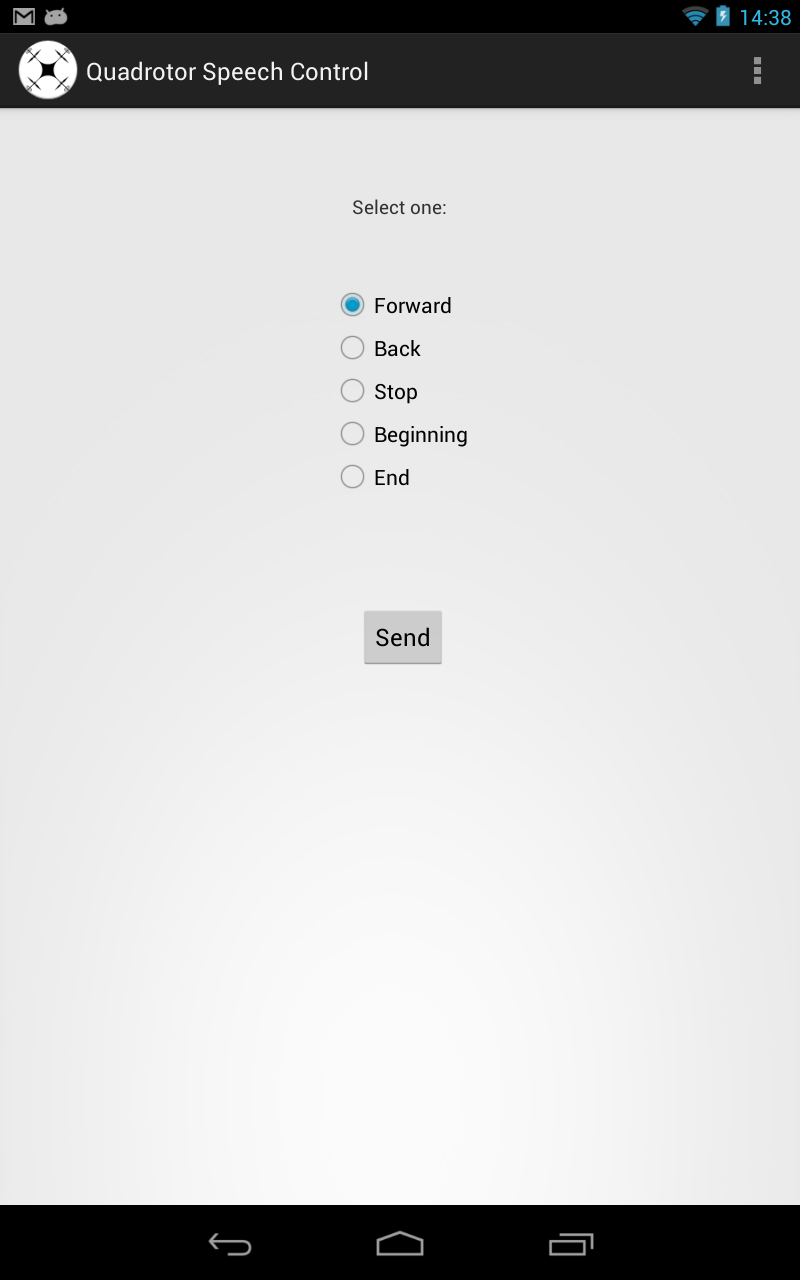
\includegraphics[scale=0.25]{figs/tablet2.png}
  \caption{Choice screen from the Android app}
  \label{fig:tablet_choice}
\end{figure}

\noindent Doing this allows us to avoid the pitfall of maximums with low probability and to be more robust during the following interactions. In fact the choice made by the user is not only used to send the proper command but also to label the interpretations of the speech recognizer and add them to the corpus.